%%%%%%%%%%%%%%%%%%%%%%%%%%EJERCICIO 9 %%%%%%%%%%%%%%%%%%%%%%%%%%%
\textbf{Ejemplo 9}\\
Amortizar en valor constante la suma de 500{.}000 COP mediante 3 pagos anuales que decrecen en 20{.}000 COP; suponga un interés del 10\% periódico anual vencido y una tasa única de corrección monetaria del 24\% nominal anual año vencido.\\			
				
\textbf{Solución 9}\\
% La tabla irá centrada
\begin{center}
	\renewcommand{\arraystretch}{1.5}% Márgenes de las celdas
	% Creación de la cuadrícula de 3 columnas
	\begin{longtable}[H]{|c|c|c|}
		% Creamos una línea horizontal
		\hline
		% Definimos el color de la primera fila
		\rowcolor[HTML]{FFB183}
		\hline
		%%%%% INICIO ASIGNACIÓN PERÍODO FOCAL %%%%%%%
		%%%%%%%%%% INICIO TÍTULO
		% Lo que se hace aquí es mezclar las 3 columnas en una sola
		\multicolumn{3}{|c|}{\cellcolor[HTML]{FFB183}\textbf{1. Asignación período focal}} \\ \hline
		%%%%%%%%%% FIN TÍTULO
		%%%%% INICIO DECLARACIÓN DE VARIABLES %%%%%%%
		\multicolumn{3}{|c|}{$pf : 0 \; \textit{pav}$} \\ \hline
		%%%%%%%%%% INICIO TÍTULO
		% Lo que se hace aquí es mezclar las 3 columnas en una sola
		\multicolumn{3}{|c|}{\cellcolor[HTML]{FFB183}\textbf{2. Declaración de variables}} \\ \hline
		%%%%%%%%%% FIN TÍTULO
		%%%%%%%%%% INICIO DE MATEMÁTICAS
		\cellcolor[HTML]{FFB183}\textbf{Valores monetarios} & 
		\cellcolor[HTML]{FFB183}\textbf{Valores no monetarios} & 
		\cellcolor[HTML]{FFB183}\textbf{Incógnitas} \\ \hline
		$VP = 500{.}000 \; \text{COP}$ & $n = 3 \; \textit{pav}$ & $R_{1} = ? \; \text{COP}$ \\ 
		$L = -20{.}000 \; \text{COP}$ & $i = 10\% \; \textit{pav}$ & $R_{2} = ? \; \text{COP}$ \\ 
		$ $ & $ $ & $R_{3} = ? \; \text{COP}$ \\ \hline
		%%%%%%%%%% FIN DE MATEMÁTICAS
		%%%%% FIN DECLARACIÓN DE VARIABLES

		\rowcolor[HTML]{FFB183}
		\hline
		\multicolumn{3}{|c|}{\cellcolor[HTML]{FFB183}\textbf{3. Diagrama de flujo de caja}} \\ \hline
		\multicolumn{3}{|c|}{ 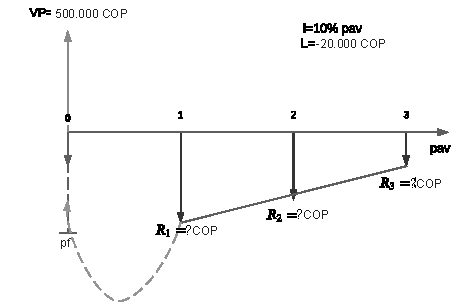
\includegraphics[trim=-78 -5 -78 -5]{7_Capitulo/img/ejemplos/9/9_1.pdf} } \\ \hline
		%%%%% INICIO FLUJO DE CAJA
		\rowcolor[HTML]{FFB183}
		\hline
		\multicolumn{3}{|c|}{\cellcolor[HTML]{FFB183}\textbf{4. Declaración de fórmulas}} \\ \hline
		%%%%%%%%%%%%% FIN INSERCIÓN DE IMAGEN
		%%%%% FIN FLUJO DE CAJA

		\multicolumn{3}{|c|}{ $VP = R\frac{1- (1+i)^{-n} }{i} + \frac{L}{i} \left( \frac{1- (1+i)^{-n} }{i} - n(1+i)^{-n}\right) $ Valor presente serie uniforme anticipada } \\ \hline
		
		%%%%%% INICIO DESARROLLO MATEMÁTICO
		\rowcolor[HTML]{FFB183}
		\hline
		%%%%%%%%%% INICIO TÍTULO
		\multicolumn{3}{|c|}{\cellcolor[HTML]{FFB183}\textbf{5. Desarrollo matemático}} \\ \hline
		%%%%%%%%%% FIN TÍTULO
		%%%%%%%%%% INICIO MATEMÁTICAS
		\multicolumn{3}{|c|}{ $500{.}000 \; \text{COP} = R\frac{1- (1+0{.}10)^{-3} }{0{.}10} + \frac{-20{.}000}{0{.}10} \left( \frac{1- (1+0{.}10)^{-3} }{0{.}10} - 3(1+0{.}10)^{-3}\right) $ } \\ 
		\multicolumn{3}{|c|}{ $R = 219{.}788{,}52 \; \text{COP}$ } \\ 
		\multicolumn{3}{|c|}{ $R_{1} = 219{.}788{,}52 \; \text{COP} \cdot (1 + 0{.}24)^{1} = 272{.}537{,}76 \; \text{COP}$ } \\ 
		\multicolumn{3}{|c|}{ $R_{2} = 199{.}788{,}52 \; \text{COP} \cdot (1 + 0{.}24)^{2} = 307{.}194{,}83 \; \text{COP}$ } \\ 
		\multicolumn{3}{|c|}{ $R_{3} = 179{.}788{,}52 \; \text{COP} \cdot (1 + 0{.}24)^{3} = 342{.}789{,}12 \; \text{COP}$ } \\ \hline
	
		%%%%%%%%%% FIN MATEMÁTICAS
		%%%%%% FIN DESARROLLO MATEMÁTICO
		%%%%%% INICIO RESPUESTA
		\rowcolor[HTML]{FFB183}
		\hline
		%%%%%%%%%% INICIO TÍTULO
		\multicolumn{3}{|c|}{\cellcolor[HTML]{FFB183}\textbf{6. Respuesta}} \\ \hline
		%%%%%%%%%% FIN TÍTULO
		%%%%%%%%%% INICIO RESPUESTA MATEMÁTICA
		\multicolumn{3}{|c|}{ 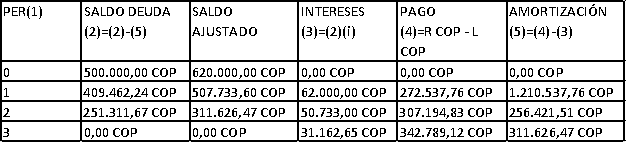
\includegraphics[trim=-78 -5 -78 -5]{7_Capitulo/img/ejemplos/9/9_2.pdf} } \\ \hline
	\end{longtable}
	% Se crean dos líneas en blanco para que no quede el siguiente texto tan pegado
	%\newline \newline % USARLO SI CREES QUE ES NECESARIO
\end{center}
%%%%%%%%%%%%%%%%%%%%%%%%%%FIN EJERCICIO 9 %%%%%%%%%%%%%%%%%%%%%%%%%%%
